\chapter[Inestabilidades en un BHL]{Radiaci\'{o}n de Hawking an\'{a}loga como una inestabilidad en un BHL}\label{cap3}

Como se introdujo en la secci\'{o}n \ref{sec:Inestabilidad} las inestabilidades son inherentes en el an\'{a}lisis de la din\'{a}mica de perturbaciones generadas en un fluido en movimiento \citep{Hydrodynamic}. Hemos descrito el campo o fluctuaci\'{o}n que se genera en el fluido a partir de los modos normales en que \'{e}ste oscila. Estos modos son ondas planas de la forma $\exp[i(kx-\omega t)]$, donde $k$ denota el número de onda espacial y $\omega$ la frecuencia temporal. Esta descripci\'{o}n es t\'{i}pica para una perturbaci\'{o}n como las ondas superficiales en un fluido (ignorando viscosidad), sonido o luz, donde usualmente $k$ y $\omega$ son reales. Pero en el vocabulario de inestabilidades hidrodinámicas, estas ondas puras se denominan \textit{ondas neutrales} y pueden ser generalizadas permitiendo que $k$ y $\omega$ sean cantidades complejas.\\

Elegir $k$ real y $\omega$ complejo significa tener una \textit{inestabilidad temporal}, que corresponde a una situación física donde se impone un forzamiento espacial al flujo, en nuestro caso es tener un perfil de velocidades para el flujo. Si hay un número de onda para el cual su frecuencia $\omega=\omega_R+i\omega_I$ sea un n\'{u}mero complejo con $\omega_I(k)>0$  entonces la perturbación crece exponencialmente y el flujo se considera linealmente inestable. En este caso, cuando $\omega_I=0$ se obtiene el caso t\'{i}pico	llamado neutral, mientras que un modo con $\omega_I<0$ se conoce como amortiguado o estable \citep{gallaire2017fluid}.\\

¿Qu\'{e} pasa en el caso general en que $k$ y $\omega$ sean complejos? Este tipo de inestabilidad espacio-temporal puede analizarse condicionando al campo $\phi$ que describe las excitaciones en el fluido a ser una funci\'{o}n de cuadrado integrable, por tanto una de las condiciones que se debe cumplir es que $\phi\rightarrow 0$ cuando $x\longrightarrow \pm \infty$. Para que esto ocurra, el n\'{u}mero de onda $k=k_R+ik_I$ con $k_I>0$ cuando $x \rightarrow -\infty$ y $k_I<0$ cuando $x \rightarrow \infty$.\\

En este cap\'{i}tulo mostraremos los resultados de \cite{2018Bermudez}, donde se considera el modelo simple para un láser de agujero negro en un condensado de Bose-Einstein (BEC), ver secci\'{o}n \ref{BHL}. Se analiza la relaci\'{o}n de dispersi\'{o}n de forma cl\'{a}sica, es decir, usando el m\'{e}todo gr\'{a}fico donde solo se permite que $k$ y $\omega$ sean reales (inestabilidad neutra), posteriormente se resuelve la misma relaci\'{o}n de dispersi\'{o}n de forma an\'{a}litica encontrando que algunos $k$ pueden tomar valores complejos. Seguido a esto se generaliza el problema a encontrar las inestabilidades espacio-temporales las cuales resultan ser los modos resonantes que se encuentran por un m\'{e}todo simple \citep{Leonhardt2007}, permitiendo as\'{i} concluir que la radiaci\'{o}n resonante en un BHL es producto de una inestabilidad.

\section{M\'{e}todo gr\'{a}fico: BHL con frecuencias reales}\label{sec:real}
Iniciemos recordando que la relaci\'{o}n de dispersi\'{o}n que deben cumplir las fluctuaciones que se crean en la configuraci\'{o}n del BHL es
\begin{equation}\label{ec:disprelation}
(\omega-vk)^2=F^2(k)=c^2k^2\left(1+\frac{k^2}{k_0^2}\right),
\end{equation}
donde dada una frecuencia $\omega$, se pueden encontrar hasta cuatro posibles soluciones para el num\'{e}ro de onda $k$ de la ec. (\ref{ec:disprelation}) por el  m\'{e}todo gr\'{a}fico o num\'erico. En la figura \ref{fig:3.1}(a) se muestran las soluciones de la relaci\'{o}n de dispersi\'{o}n para dos velocidades: una subs\'{o}nica $|v_1|<c$ y otra supers\'{o}nica $|v_2|>c$. Con la velocidad subs\'{o}nica $v_1$ con este m\'{e}todo se encuentran dos soluciones (formalmente ser\'{i}an cuatro soluciones, pero dos de ellas son complejas y se analizar\'{a}n en la siguiente secci\'{o}n). Con la velocidad supers\'{o}nica $v_2$ se encuentran las cuatro soluciones.\\
\begin{figure}
   \centering
   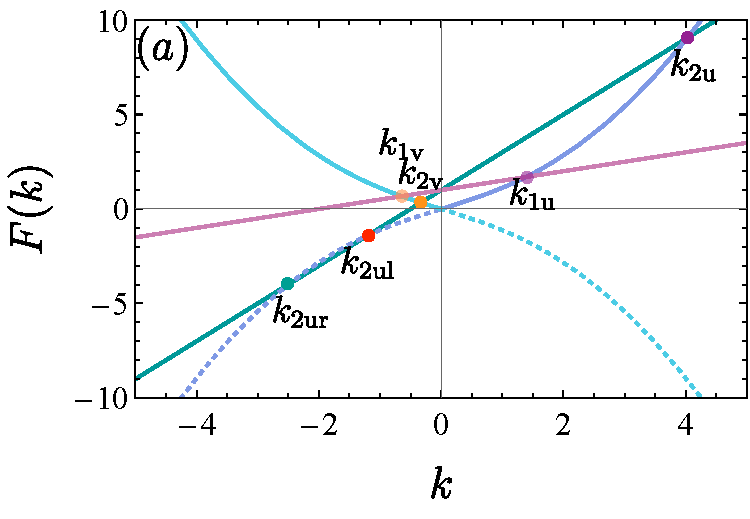
\includegraphics[height=5cm]{f31a.pdf}%
   \hspace{0.1cm}% add some horizontal spacing
   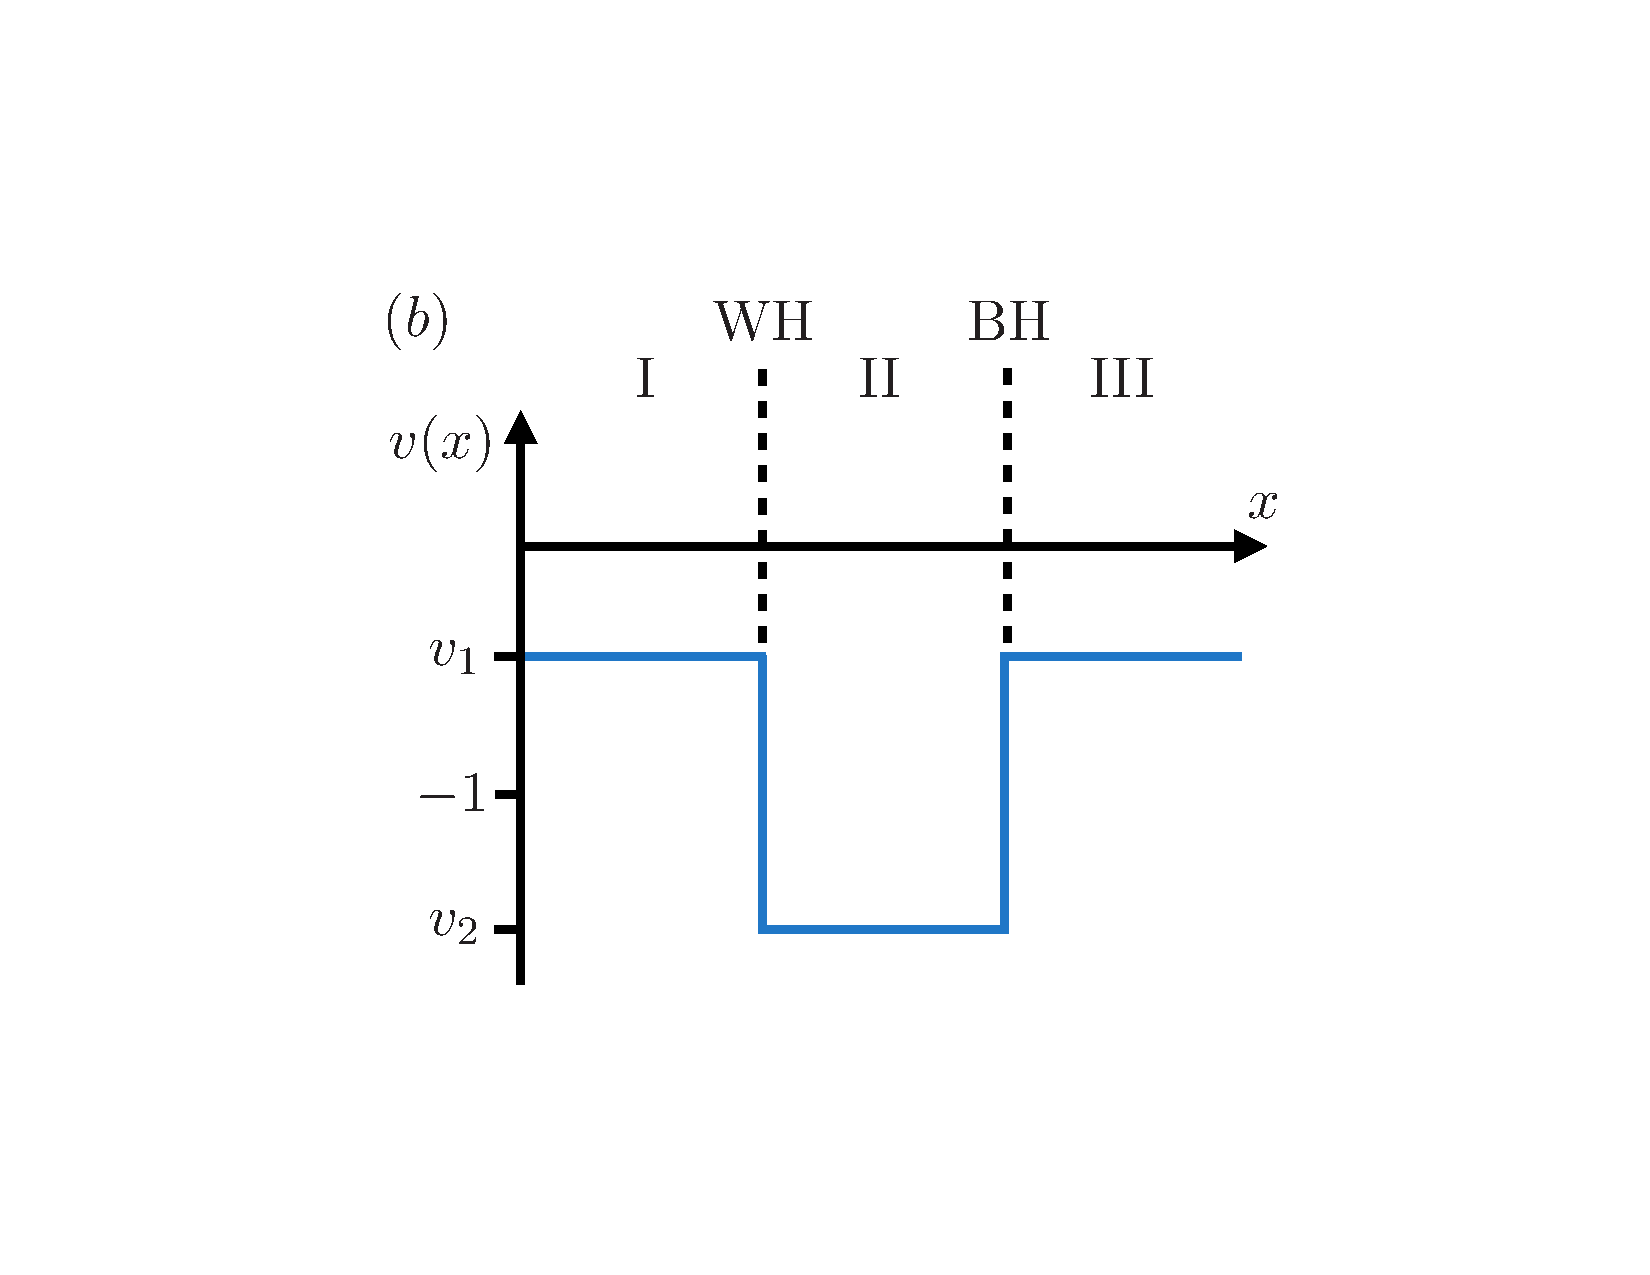
\includegraphics[height=6cm]{Fig21.pdf}%
   \caption{(a) Relaci\'{o}n de dispersi\'{o}n en el marco com\'{o}vil. En morado se encuentra la rama que contiene modos contrapropagantes, mientras de azul la rama con modo copropagantes. La solución gráfica para dos perfiles de velocidad: una subsónica $v_1$ (rosa) y otra supersónica $v_2$ (verde). Aquí $v_1= -1$, $k_0 = 2$, $c = 1$, $v_2= - 2$, y $\omega=1$. (b) Perfil de velocidades del fluido $v(x)$ para las tres regiones, I y III con velocidad subs\'{o}nica y II con velocidad supers\'{o}nica \citep{2018Bermudez}.} 
   \label{fig:3.1}
\end{figure}

Los modos $k$ que son soluci\'{o}n tambi\'{e}n se nombran por los sub\'{i}ndice u que indica que el modo es contrapropagante, o que se mueven en direcci\'{o}n opuesta al fluido (recordar que el fluido por convenci\'{o}n se mueve hacia la izquierda); con $k>0$, existen tanto para $v_1$ como para $v_2$ modos contrapropagantes. Para $k<0$ solo para $v_2$ se tienen los modos $\text{ul}$ y $\text{ur}$, que se distinguen porque el primero se mueve hacia la izquierda y el segundo hacia la derecha en el marco com\'{o}vil. Las etiquetas con sub\'{i}ndice $v$ indican modos copropagantes y existen solo cuando $k<0$ y se mueven en la misma direcci\'{o}n del fluido.\\

El BHL es una configuraci\'{o}n donde el flujo de velocidad cambia de una velocidad subs\'{o}nica $v_1$  (región I) a una supers\'{o}nica $v_2$ (región II) en una regi\'{o}n finita $L$ del espacio  y regresa a una velocidad $v_1$ (región III). Su parametrizaci\'{o}n est\'{a} dada en el perfil de velocidad que se representa en la figura \ref{fig:3.1}(b). Como se mencion\'{o} en la secci\'{o}n \ref{BHL}, la regi\'{o}n supers\'{o}nica representa el interior de la cavidad y es donde la radiaci\'{o}n de Hawking se amplificar\'{a}. Para cualquier $0<\omega<ck_0$ existe un dominio de $v_1$ y $v_2$ donde las soluciones en el marco com\'{o}vil tienen el comportamiento mostrado en la figura \ref{fig:3.1}(a). Los puntos donde el flujo de velocidad cambia son llamados horizontes y la unica condici\'{o}n que se debe cumplir es que $|v_1|<c<|v_2|$. En la figura \ref{fig:3.1}(b) al lado izquierdo tenemos un horizonte de agujero blanco (WH) y a la derecha, un horizonte de agujero negro (BH).

\subsection{Direcci\'{o}n de viaje}
La direcci\'{o}n de viaje de las autofunciones del problema est\'{a} dada por:
\begin{equation}
v_g=\frac{\partial \omega}{\partial k}=c\frac{1+2k^2/k_0^2}{\sqrt{1+k^2/k_0^2}},
\end{equation} 
y considerando la velocidad del flujo negativa para cada una de las regiones $v_1$ y $v_2$, se obtienen las velocidades de grupo en el marco del laboratorio para lo modos contrapropagantes (u) y copropagantes (v)
\begin{align}
v_{\text{1u}}(k)&=v_g(k)+v_1,\hspace{2cm} v_{\text{1v}}(k)=-v_g(k)+v_1,\\
v_{\text{2u}}(k)&=v_g(k)+v_2,\hspace{2cm} v_{\text{2v}}(k)=-v_g(k)+v_2.
\end{align}
\begin{figure}\centering
	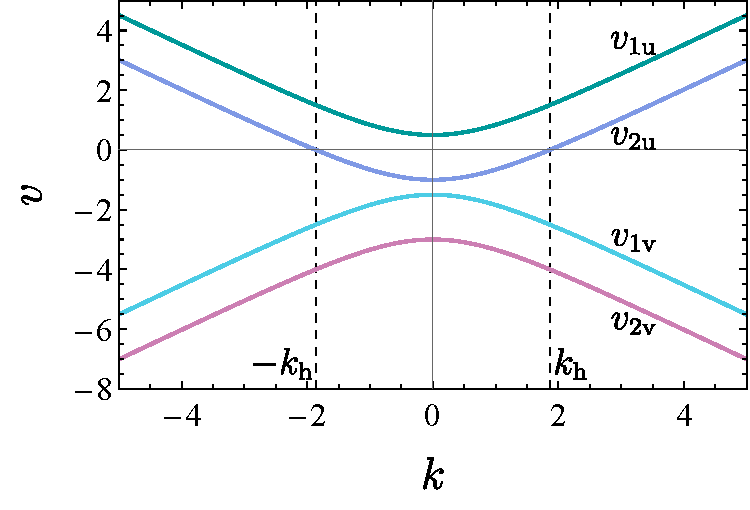
\includegraphics[scale=0.7]{f32}
	\caption{Velocidad de grupo en el marco de laboratorio para los modos $k$. Para $v_1=-1/2$ y $v_2=-2.$ De mayor a menor son: $v_{\text{1u}}$ (azul), $v_{\text{2u}}$ (naranja), $v_{\text{1v}}$ (verde), $v_{\text{2v}}$ (rojo). Los horizontes $\pm k_\text{h}$ están marcados por líneas verticales entrecortadas \cite{2018Bermudez}.}\label{fig:3.2}
\end{figure}

Cada una de estas velocidades son mostradas en la figura \ref{fig:3.2}. Como es de esperar, la velocidad de los modos copropagantes (v) siempre es negativa (son modos que se mueven con el flujo). Para los modos contrapropagantes (modos (u)), en la regi\'{o}n subs\'{o}nica ($v_1$), la velocidad es siempre positiva, pero en la regi\'{o}n supers\'{o}nica ($v_2$) existe una regi\'{o}n finita en los valores del n\'{u}mero de onda $k$ donde la velocidad es negativa. La regi\'{o}n de flujo opuesto para $v_{2\text{u}}$ está marcada por líneas discontinuas en la figura \ref{fig:3.2} y los valores límites se conocen como horizontes $\pm k_{\text{h}}$. Para cálculos numéricos se usar\'{a}n unidades adimensionales. En este caso, significa normalizar las velocidades $v$ con respecto a la velocidad del sonido, es decir, $v / c$.
\subsection{Horizonte}\label{Horizonte Acustico}

Hemos definido el horizonte como el l\'{i}mite espacial que separa dos regiones del espacio-tiempo donde puede existir el campo o fluctuaci\'{o}n. Este l\'{i}mite f\'{a}cilmente se encuentra al igualar la velocidad de la fluctuaci\'{o}n con la velocidad del medio en movimiento. En el caso de no tener dispersi\'{o}n, como es el caso astrof\'{i}sico, el horizonte est\'{a} bien definido, es decir, cualquier frecuencia del campo siente el horizonte en el mismo lugar del espacio-tiempo, pero cuando se tiene dispersi\'{o}n como en el an\'{a}logo ac\'{u}stico o m\'{a}s adelante en el caso \'{o}ptico, el horizonte es difuso en el sentido que para cada frecuencia existe un horizonte.\\

Teniendo en cuenta lo anterior, definimos el horizonte $k_\text{h}$ como el n\'{u}mero de onda para el cual la velocidad de grupo  $v_g$ de los modos contrapropantes es igual a la velocidad del flujo externo $v$. Esto es solo posible para los modos contrapropagantes (u) en la regi\'{o}n supers\'{o}nica ($v_2$) la cual es solo la curva para $v_{2\text{u}}(k)$ que se hace cero para ciertos valores $k_{\text{h}}$, ver figura \ref{fig:3.2}. La anterior definici\'{o}n se expresa como:
\begin{equation}
v_{\text{2u}}(k)|_{k=k_{\text{h}}}=0.
\end{equation}

 La solución general para este valor es:
 \begin{equation}\label{ec:horizonte}
 k_{\text{h}}=\pm\frac{k_0}{2^{3/2}}\sqrt{\frac{v^2}{c^2}-4\pm\frac{v}{c}\sqrt{\frac{v^2}{c^2}+8,}}
 \end{equation}
este es el mismo resultado en contrado en \citep{2012Larre}, \citep{2009RParentani}. Para una velocidad suficientemente alta hay dos soluciones reales, por ejemplo, para $v_2=-2$ se obtienen los valores $k_{\text{h}}$ que se muestran en la figura \ref{fig:3.2}. Para velocidades bajas no hay soluciones reales, como en el caso de $v_1$ en este ejemplo. Esto es correcto, ya que no hay horizonte para velocidades subsónicas. Observe que en este sistema creado en condensados la velocidad supers\'{o}nica y subs\'{o}nica no tienen restricci\'{o}n en sus valores, salvo que sea $|v_1|<c$ y $|v_2|>c$.


\subsection{Velocidad trans\'{o}nica}
Como se acaba de observar, dadas $\omega$ y $k_0$ existe una velocidad mínima necesaria para alcanzar el horizonte, esta no es la velocidad del sonido $c$, sino la velocidad mínima para la cual las soluciones $k_{2\text{ur}}$ y $k_{2\text{ul}}$ existen (son reales) e iguales, esta es la velocidad\textit{ transónica} $v_t$. Esta velocidad define las regiones subsónica $(v_t <v <0)$ y supersónica $(v <v_t)$ para cada $\omega$, y existe por que se toma en cuenta la dispersi\'{o}n del medio donde se propagan los modos.\\

Esta velocidad puede ser encontrada anal\'{i}ticamente con una funci\'{o}n auxiliar $q(k_0,\omega)$ definida como
\begin{equation}
q^3=729\frac{k_0^4c^4}{\omega^4}+270\frac{k_0^2c^2}{\omega^2}+3^{3/2}\frac{k_0c}{\omega}\Bigl(27\frac{k_0^2c^2}{\omega^2}-4\Bigr)^{3/2}-2,
\end{equation}
con 
\begin{equation}
v_t^2=c^2\Bigl(1+\frac{\omega^2}{3k_0^2c^2}(2^{-1/3}q-1)+\frac{2^{1/3}}{3q}(\frac{\omega^2}{k_0^2c^2}+54)\Bigr)
\end{equation}
 y para este caso, tomando el negativo de la ra\'{i}z cuadrada. Para $c=1$, $k_0=2$, y $\omega=1$, se obtiene $v_t=-1.9002.$
 
 
\section{M\'{e}todo anal\'{i}tico: BHL con frecuencias complejas}\label{sec:compleja}
En esta secci\'{o}n se aplicar\'{a} la teoría de inestabilidades al BHL, para ello obtendremos primero las ra\'ices de la ec. (\ref{ec:disprelation}) para $\omega$ real y $k$ complejo y luego generalizamos las soluciones para números de onda $k$ y frecuencias $\omega$ complejos teniendo as\'{i} las inestabilidades espacio-temporales. Recordemos que la forma can\'{o}nica de una ecuaci\'{o}n de cuarto orden como la de la relaci\'{o}n de dispersi\'{o}n dada en la ec. (\ref{ec:disprelation}) es
\begin{equation}
k^4+dk^3+ek^2+fk+g=0,
\end{equation}
con los siguientes coeficientes
\begin{align}
d=0, \hspace{0.5cm} e=\Bigl(1-\frac{v^2}{c^2}\Bigr)k_0^2, \hspace{0.5cm} f=\frac{2v\omega k_0^2}{c^2}, \hspace{0.5cm} g=\frac{-\omega^2 k_0^2}{c^2}.
\end{align}
Este tipo de ecuaciones con $d=0$ pueden ser reducidas a una ecuaci\'{o}n auxiliar  c\'{u}bica
\begin{equation}
k^3+\frac{e}{2}k^2+\frac{e^2-4g}{16}k-\frac{f^2}{64}=0,
\end{equation}
donde sus soluciones $p_1,p_2$ y $p_3$ otorgan la soluci\'{o}n a la ecuaci\'{o}n de cuarto orden dada en la ec. (\ref{ec:disprelation}) inicial
\begin{align}
k_1&=\sqrt{p_1}+\sqrt{p_2}+\sqrt{p_3}, \quad k_2&=\sqrt{p_1}-\sqrt{p_2}-\sqrt{p_3},\\
k_3&=-\sqrt{p_1}+\sqrt{p_2}-\sqrt{p_3}, \quad k_4&=-\sqrt{p_1}-\sqrt{p_2}+\sqrt{p_3}.
\end{align}
 Aunque las soluciones explícitas son demasiado largas para escribirlas, se pueden usar en cálculos analíticos. De esta manera se obtienen cuatro soluciones para cada flujo de velocidad, i.e., para cada regi\'{o}n del BHL. El comportamiento de las cuatro soluciones complejas cuando var\'{i}a la velocidad del flujo se muestra en la figura \ref{fig:3.4}. En esta gr\'{a}fica se marca la velocidad trans\'{o}nica $v_t$ con una l\'{i}nea vertical que indica en que velocidad se vuelven complejas las soluciones $k_{\text{ur}}$ y $k_{\text{ul}}$ . Las soluciones del n\'{u}mero de onda $k$ para la regi\'{o}n subsónica $v_1$ y supersónica $v_2$ mostradas en las figuras \ref{fig:2.1} y \ref{fig:3.4} se retoman en la figura \ref{fig:3.5}, que es la representaci\'{o}n del espacio complejo del n\'{u}mero de onda.\\

Comparando con las soluciones del método numérico, se obtienen los mismos resultados reales, cuatro en la región supersónica y dos en la subsónica. Además, se obtienen dos soluciones extras, las cuales son complejas conjugadas entre sí y no aparecen en el tratamiento habitual del sistema BHL mostrado en la secci\'{o}n \ref{sec:real}. Estas dos soluciones adicionales en la parte subsónica tienen n\'{u}mero de onda $k$ complejo, lo que genera un aumento o disminuci\'{o}n exponencial para ciertas regiones del espacio.
\begin{equation}\label{prueba1}
\exp[ikx]=\exp[i(k_R+ik_I)x]=\exp[-k_Ix]\exp[ik_Rx].
\end{equation}
Tal que, si $k_I>0$, la soluci\'{o}n decae a la derecha ($x>0$), y si $k_I<0$, la soluci\'{o}n decae a la izquierda ($x<0$).
\begin{center}
\begin{figure}[h]
\begin{minipage}[c]{0.5\textwidth}
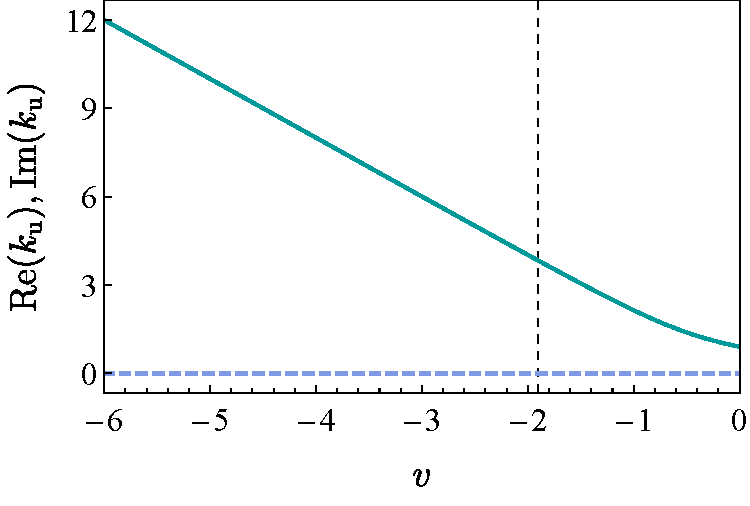
\includegraphics[width=7cm]{p1}
  \end{minipage}%                       
\begin{minipage}[c]{0.5\textwidth}
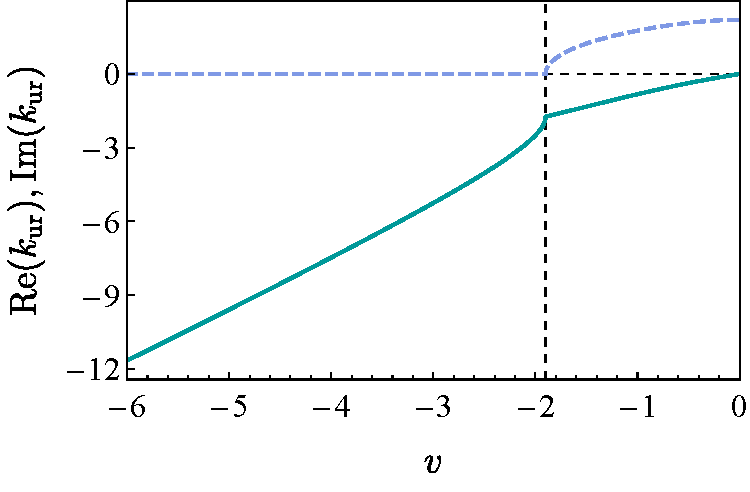
\includegraphics[width=7cm]{p2}
\end{minipage}\\[20pt]                 
\begin{minipage}[c]{0.5\textwidth}
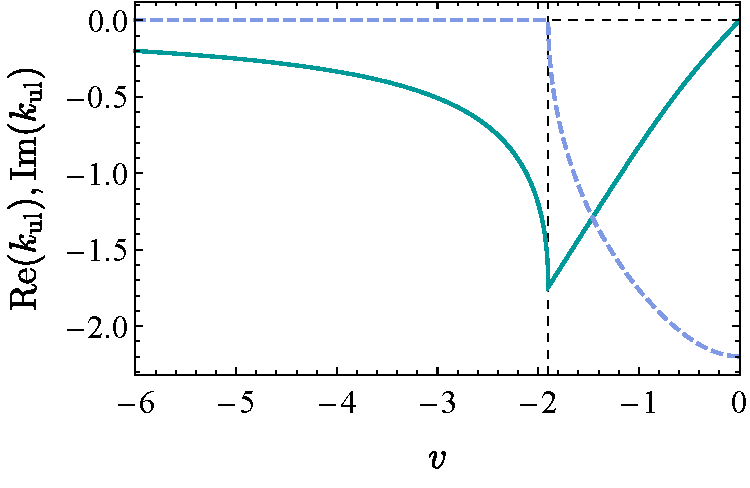
\includegraphics[width=7cm]{p3}
  \end{minipage}%
\begin{minipage}[c]{0.5\textwidth}
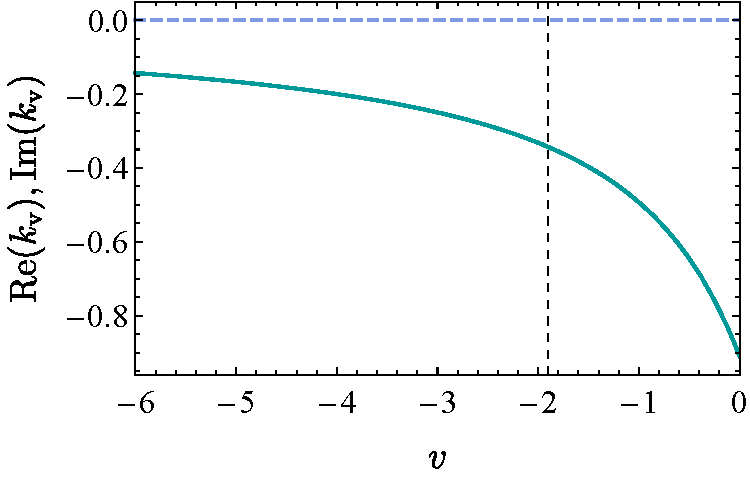
\includegraphics[width=7cm]{p4}
\end{minipage}\\[20pt] 
\caption{Las cuatro soluciones analíticas en  funci\'{o}n de la velocidad del flujo variable $v$, la parte real (l\'{i}nea continua verde) y la parte imaginaria (l\'{i}nea discontinua morada) se muestran para $k_0 = 2$ y $\omega=1$. La vertical discontinua corresponde a la velocidad transónica $v_t=1.9002$. Podemos ver que $k_\text{u}$ y $k_\text{v}$ son reales para todas las velocidades, mientras que $k_{\text{ur}}$ y $k_{\text{ul}}$ son reales solo para velocidades supersónicas \citep{2018Bermudez}.}\label{fig:3.4}   
\end{figure}
\end{center}
\begin{figure}[h]
\centering
	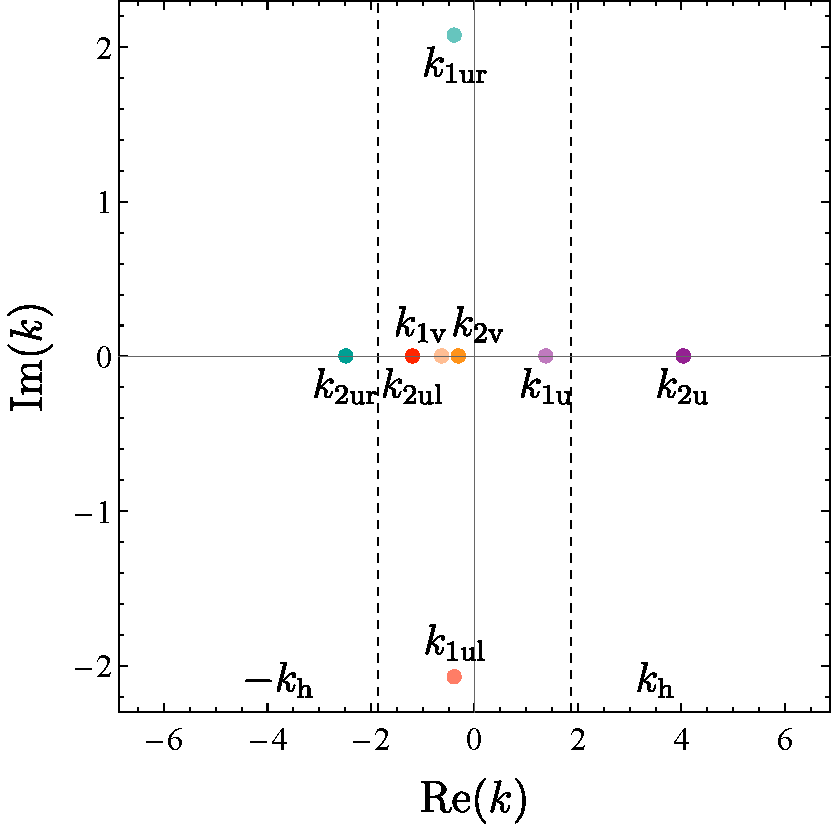
\includegraphics[height=7cm]{f34}
	\caption{Soluciones analíticas para $v_1=-1/2$ y $v_2=-3$ en el espacio k complejo. Se obtienen las seis soluciones reales originales más dos complejas nuevas completando las ocho soluciones al problema, cuatro pertenecen a la regi\'{o}n subs\'{o}nica y otras cuatro a la supers\'{o}nica. Las líneas en $k_h$ ayudan a encontrar la dirección de desplazamiento de los modos: $k_{2\text{u}}$, $k_{2\text{ur}}$ y $k_{2\text{ul}}$ \citep{2018Bermudez}.}\label{fig:3.5}
\end{figure}


\subsection{Descripci\'{o}n cualitativa y cuantitativa}
Ahora se desea encontrar las inestabilidades espacio-temporales en el BHL, es decir, encontrar las funciones propias del sistema con frecuencias complejas $\omega=\omega_R+i\omega_I$, con la parte imaginaria positiva, esto implica que la amplitud incrementa exponencialmente con el tiempo
\begin{equation}
\exp[-i\omega t]=\exp[-i(\omega_R+i\omega_I)t]=\exp[\omega_It]\exp[-i\omega_Rt].
\end{equation}
Al tomar la configuraci\'{o}n del BHL como un todo se considera la situación donde los únicos modos permitidos en la regi\'{o}n subs\'{o}nica sean aquellos que decaen exponencialmente lejos de la cavidad. Del comportamiento de las soluciones para los modos $k$ mostradas en la figura \ref{fig:3.5}, se observa que la soluci\'{o}n etiquetada como $k_{1\text{ur}}$ decae exponencialmente a la derecha ($x\rightarrow \infty$) y $k_{1\text{ul}}$ (complejo conjugado de $k_{\text{1ur}}$) decae exponencialmente a la izquierda  ($x\rightarrow -\infty$).
Lo anterior se puede resumir de manera formal de la siguiente manera: Si dividimos el campo cu\'{a}ntico $\phi$ en tres regiones I, II y III, en cada regi\'{o}n, el campo $\phi$ est\'{a} definido por
\begin{align}
\phi_I=\textbf{A}\cdot \exp(i\textbf{k}_1x),\hspace{1cm}\phi_{II}=\textbf{B}\cdot \exp(i\textbf{k}_2x)\hspace{1cm}\phi_{III}=\textbf{C}\cdot \exp(i\textbf{k}_1x),
\end{align}
donde
\begin{align}
\textbf{A}=(A_1,A_2,A_3,A_4),\hspace{1cm}\textbf{B}=(B_1,B_2,B_3,B_4),\hspace{1cm}\textbf{C}=(C_1,C_2,C_3,C_4),
\end{align}
y
\begin{align}
\nonumber \exp(i\textbf{k}_1x)=&(\exp(ik_{11}x),\exp(ik_{12}x),\exp(ik_{13}x),\exp(ik_{14}x)),\\
\exp(i\textbf{k}_2x)=&(\exp(ik_{21}x),\exp(ik_{22}x),\exp(ik_{23}x),\exp(ik_{24}x)).
\end{align}
En la configuraci\'{o}n del l\'{a}ser, los modos entrantes y salientes están permitidos siempre que el campo $\phi$ sea una funci\'{o}n de cuadrado integrable, raz\'{o}n  por la cual en el parr\'{a}fo anterior se pide que su comportamiento sean exponenciales que decaen fuera de la cavidad. Esto significa que la configuración de BHL es
$A_1 = A_2 = C_3 = C_4 = 0$, como se indica en la figura \ref{fig:3.6}. Los otros coeficientes se deben encontrar para definir por completo el campo cu\'{a}ntico en la configuraci\'{o}n BHL.


\begin{figure}\centering
	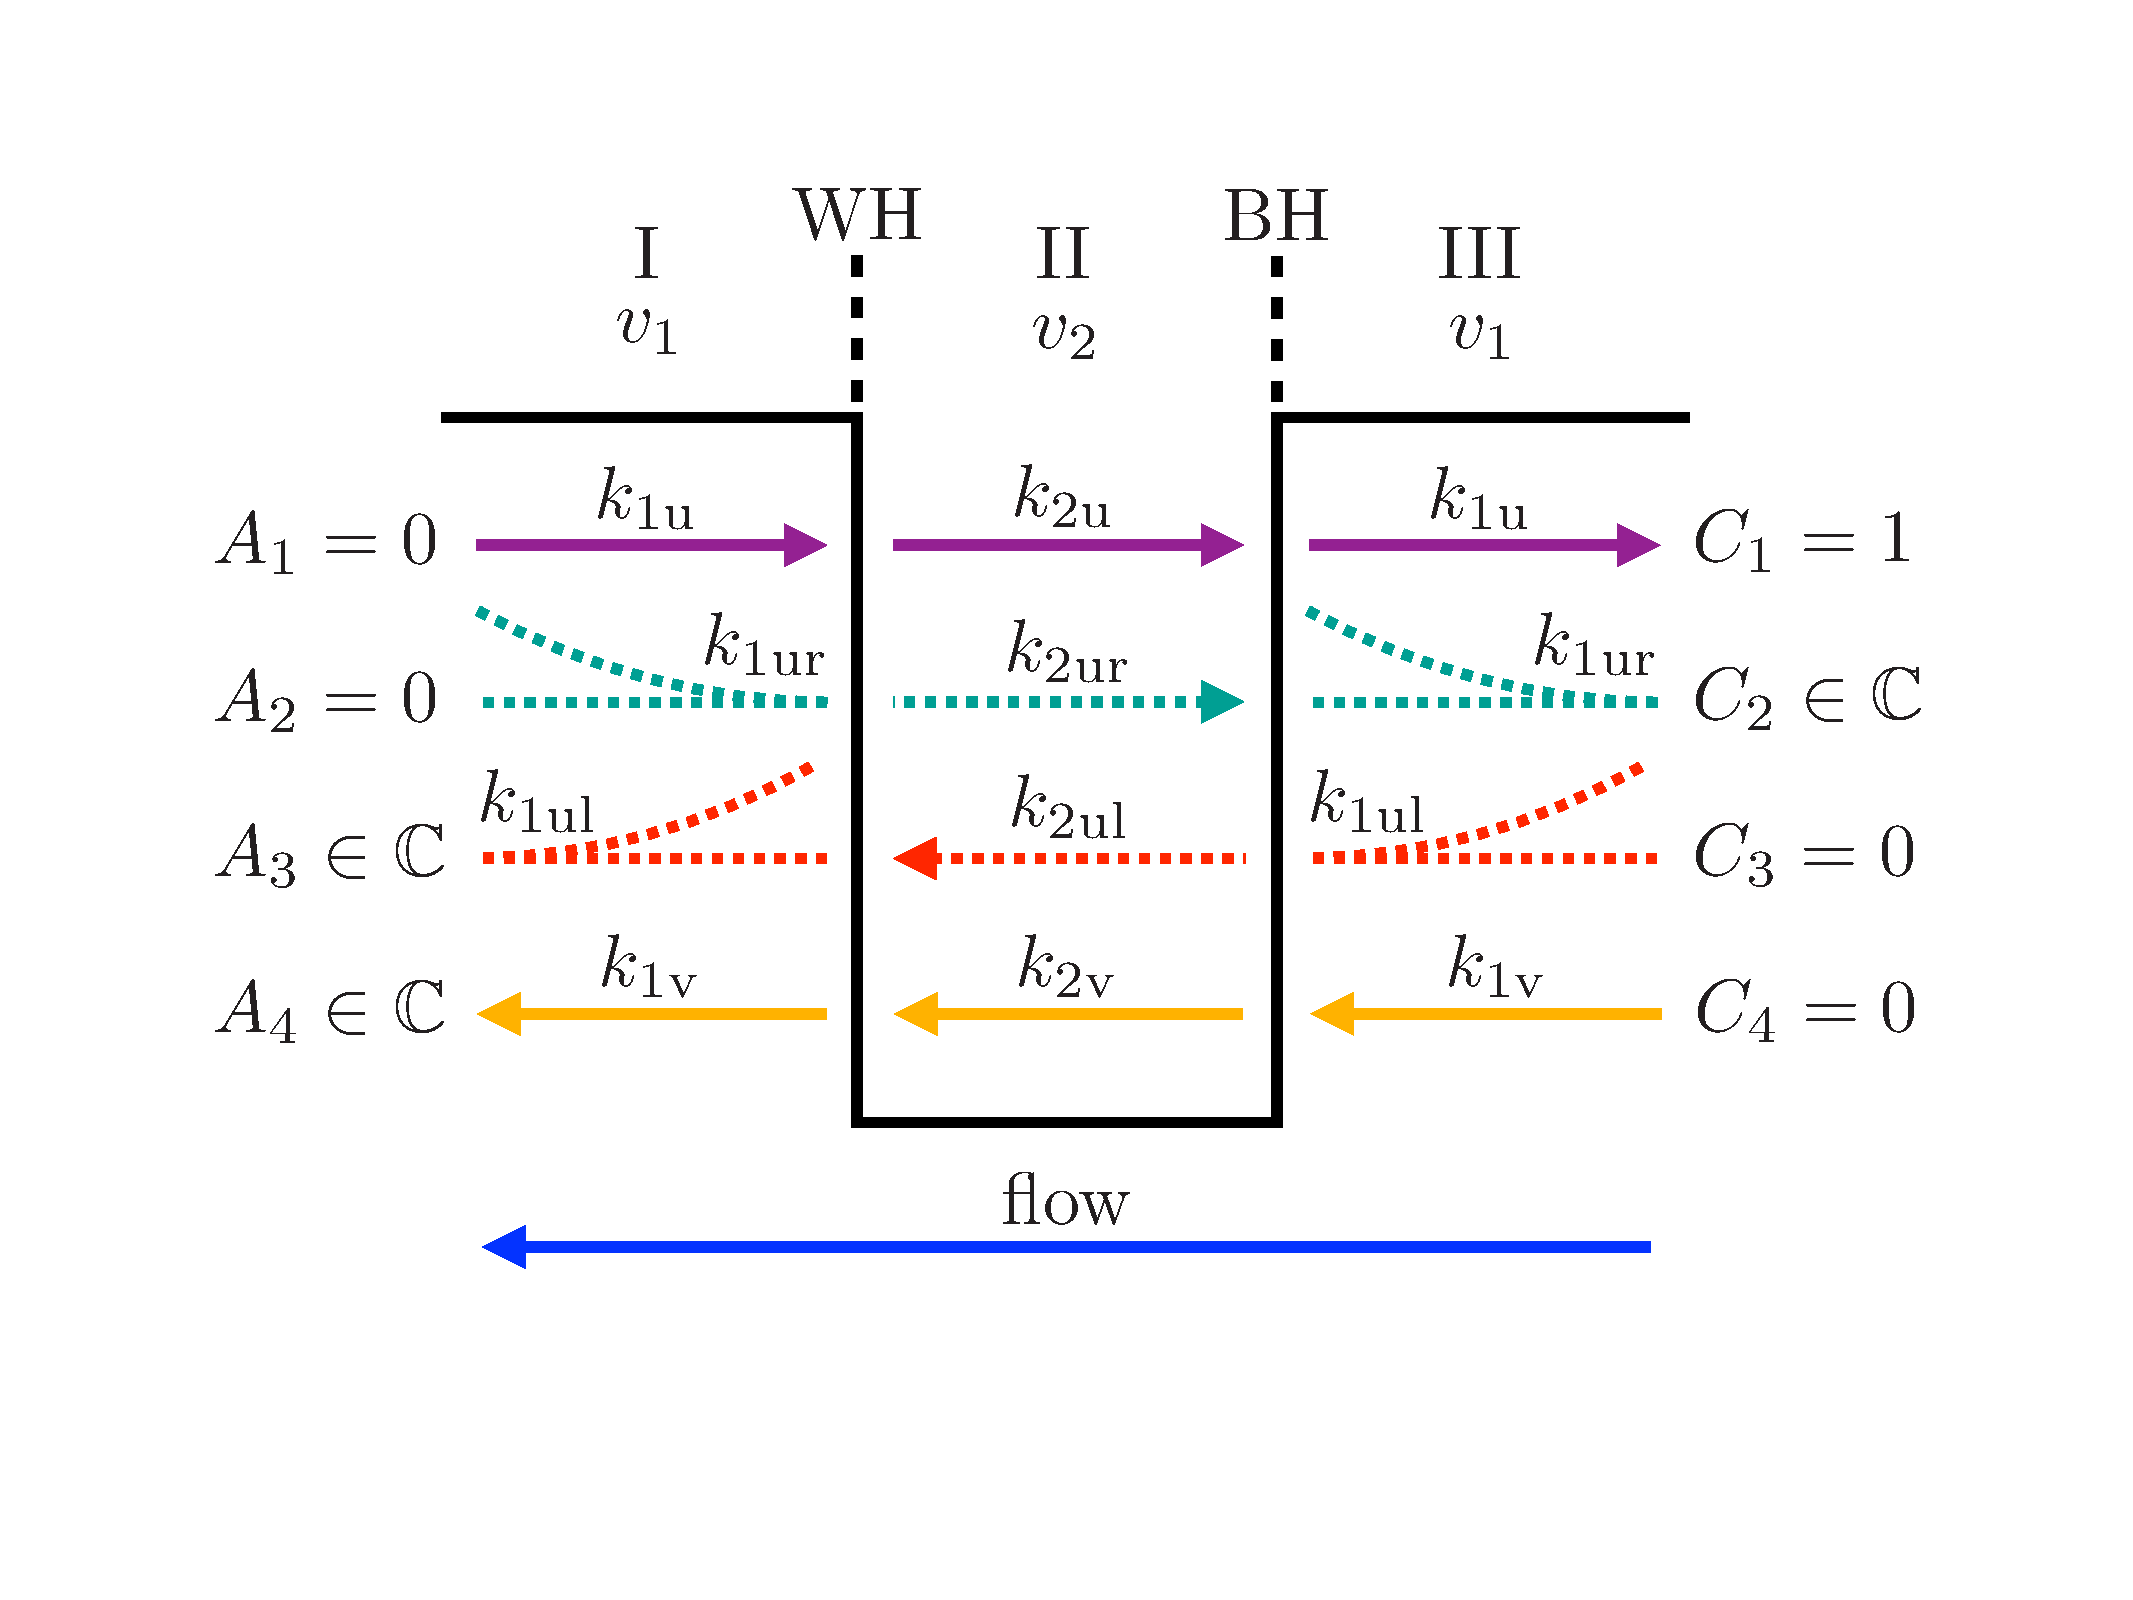
\includegraphics[height=8cm]{F35}
	\caption{Diagrama de modos de una BHL con inestabilidades. Los modos $k_{1\text{ur}}$ y $k_{1\text{ul}}$ son exponencialmente decayentes o crecientes en alguna de las regiones subs\'{o}nicas. Los coeficientes mostrados $A_j$ y $C_j$ describen la soluci\'{o}n para que el campo $\phi$ sea una funci\'{o}n de cuadrado integrable \citep{2018Bermudez}.}\label{fig:3.6}
\end{figure}

\subsection{Matriz de transferencia}\label{matriztransferencia}
Para resolver este problema se aplicar\'{a} el método de matriz de transferencia. Se puede emplear este método porque el perfil de velocidad es constante en todas las regiones excepto en las interfaces, donde se debe condicionar la continuidad del campo cuántico $\phi(x)$ y sus tres primeros derivadas $\phi'(x), \phi''(x),\phi'''(x)$ (ya que tenemos una ecuación diferencial de cuarto orden, la ec. (\ref{ec:dinamica})).\\
Definiendo las matrices de transferencia o salto de la región I a la regi\'{o}n II como ($M_1$) y de la regi\'{o}n II a la regi\'{o}n III como ($M_2$) usamos las matrices auxiliares $m_1$ y $m_2$ cuyas entradas ser\'{a}n coeficientes del campo y sus derivadas ($\phi(x),\phi'(x), \phi''(x),\phi'''(x)$)
\begin{eqnarray}
m_1=\begin{pmatrix}
1 & 1 & 1 & 1 \\ 
ik_{11} &ik_{12}  & ik_{13} &ik_{14} \\ 
-k_{11}^2 &- k_{12}^2 &-k_{13}^2  &-k_{14}^2 \\ 
 -ik_{11}^3&  -ik_{12}^3& - ik_{13}^2 & -ik_{14}^3
\end{pmatrix},\hspace{0.2cm}m_2=\begin{pmatrix}
1 & 1 & 1 & 1 \\ 
ik_{21} &ik_{22}  & ik_{23} &ik_{14} \\ 
-k_{21}^2 &- k_{22}^2 &-k_{23}^2  &-k_{24}^2 \\ 
 -ik_{21}^3&  -ik_{22}^3& - ik_{23}^2 & -ik_{24}^3
\end{pmatrix}.
\end{eqnarray} 
El primer sub\'{i}ndice en $k_{ij}$ corresponde a la velocidad $v_1$ o $v_2$, el segundo especifica la soluci\'{o}n de 1-4. Es posible seleccionar cualquier orden para las soluciones de $k$ siempre y cuando se mantenga el orden escogido, aqu\'{i} se ha ordenado como $\text{u}$, $\text{ur}$, $\text{ul}$ y $\text{v}$ como se muestra en la figura \ref{fig:3.6}. Entonces las matrices de tranferencia son simplemente 
\begin{align}
M_1=m_2^{-1} m_1, \hspace{2cm}M_2=m_1^{-1} m_2=M_1^{-1},
\end{align}
también es conveniente definir las matrices de propagación para trasladar la solución entre las interfaces de la cavidad. \'{E}stas son
\begin{align}
\nonumber P_L&=\text{diag}(\exp(-ik_{21}L),\exp(-ik_{22}L),\exp(-ik_{23}L),\exp(-ik_{24}L)),\\
P_R&=\text{diag}(\exp(ik_{21}L),\exp(ik_{22}L),\exp
(ik_{23}L),\exp(ik_{24}L)).
\end{align}
Finalmente, la matriz de transferencia $(M)$ de la regi\'{o}n III a la regi\'{o}n I est\'a dada por

\begin{align}\label{matrizM}
M=M_1P_LM_2=m_2^{-1}m_1P_Lm_1^{-1}m_2.
\end{align}
De manera similar, para pasar de la regi\'{o}n III a la regi\'{o}n I se tiene $M^{-1}$. Usando $M$, se pueden tener los coeficientes $\textbf{A}$ en t\'{e}rminos de los $\textbf{C}$, a trav\'{e}s de
\begin{equation}
\phi_I=M\phi_{III}.
\end{equation} 
Para cada $\omega$ existir\'{a} un conjunto de cuatro n\'{u}meros de onda $k$ en la regi\'{o}n subs\'{o}nica $\textbf{k}_1$ y otros cuatro en la regi\'{o}n supers\'{o}nica $\textbf{k}_2$, este problema se puede resolver analíticamente. A partir de los cuatro coeficientes $\textbf{C}$ (o$\textbf{ A}$) para cualquier frecuencia compleja se pueden determinar los ocho números de onda complejos correspondientes
$\textbf{k}_1(\omega)$ y $\textbf{k}_2(\omega)$ y finalmente calcular los cuatro coeficientes\textbf{ A} (o \textbf{C}). 
\section{Estados confinados}\label{sec:comp}
Definimos un modo inestable del láser  como un modo de la cavidad donde el campo $\phi(x)$ es una funci\'{o}n de cuadrado integrable con $\omega_I>0$. Esta es la situación mostrada en la figura \ref{fig:3.6}, donde $A_1 = A_2 = C_3 = C_4 = 0$. Iniciando con $\phi_{III}(x)$ dado por los coeficientes $\textbf{C} = (1,\rho, 0, 0)$ con $\rho \in \mathbb{C}$. Con esto, se obtiene $\phi_I(x)$ usando el método de matriz de transferencia. La solución con un coeficiente nulo se puede encontrar analíticamente, pero con un segundo, el problema tiene que ser resuelto numéricamente. Por ejemplo, si se toma $v_1 =-1 / 2$, $v_2=-3$ y $L=1$, hay una solución única dada por $\omega_l= 2.4613 + i0.5667$, donde el subíndice \textit{l} indica que es un modo inestable. El campo cuántico $\phi$ para estas condiciones que el  perfil de velocidades mostrado figura \ref{fig:3.1}(b), junto a otro perfil de velocidades dado por $v_1=-1/2$ y $v_2=-3$, se muestran en la figura \ref{fig:3.7}. Aqu\'{i} se grafica el m\'odulo del campo $|\phi(x)|$, su  parte real e imaginaria, mostrando que cada una de sus partes son funciones continuas y decaen lejos de la cavidad. También se verifica que las tres primeras derivadas son continuas en los horizontes.\\

\begin{center}
\begin{figure}[h]
\begin{minipage}[c]{0.5\textwidth}
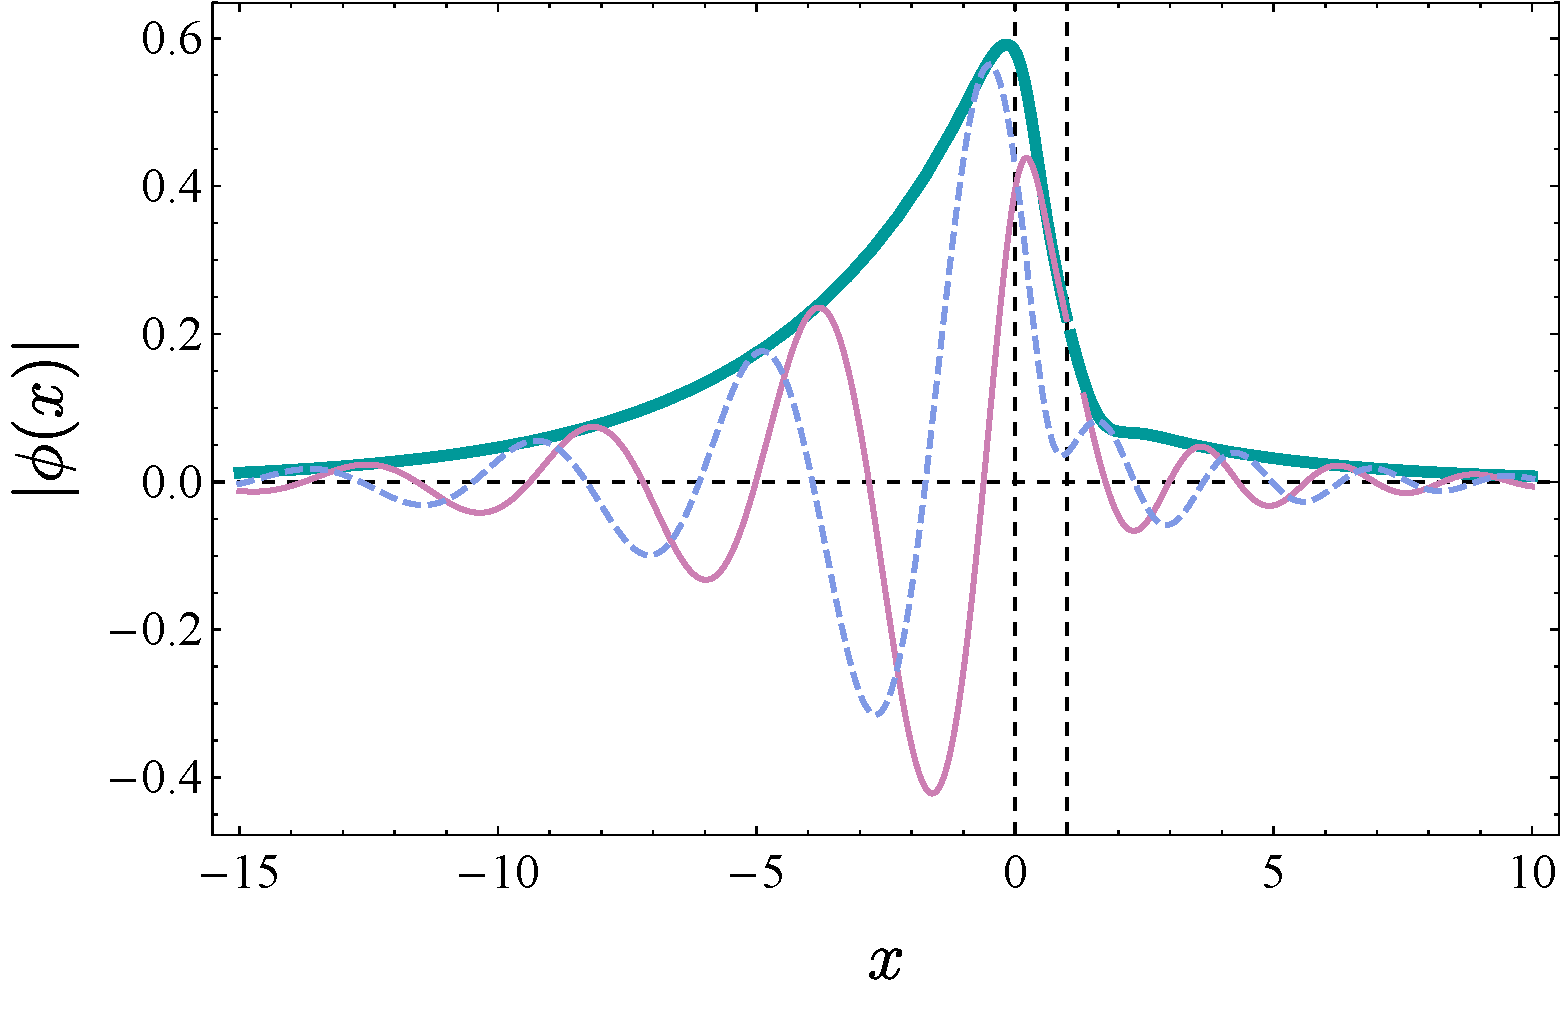
\includegraphics[width=7cm]{f36a}
  \end{minipage}%                       
\begin{minipage}[c]{0.5\textwidth}
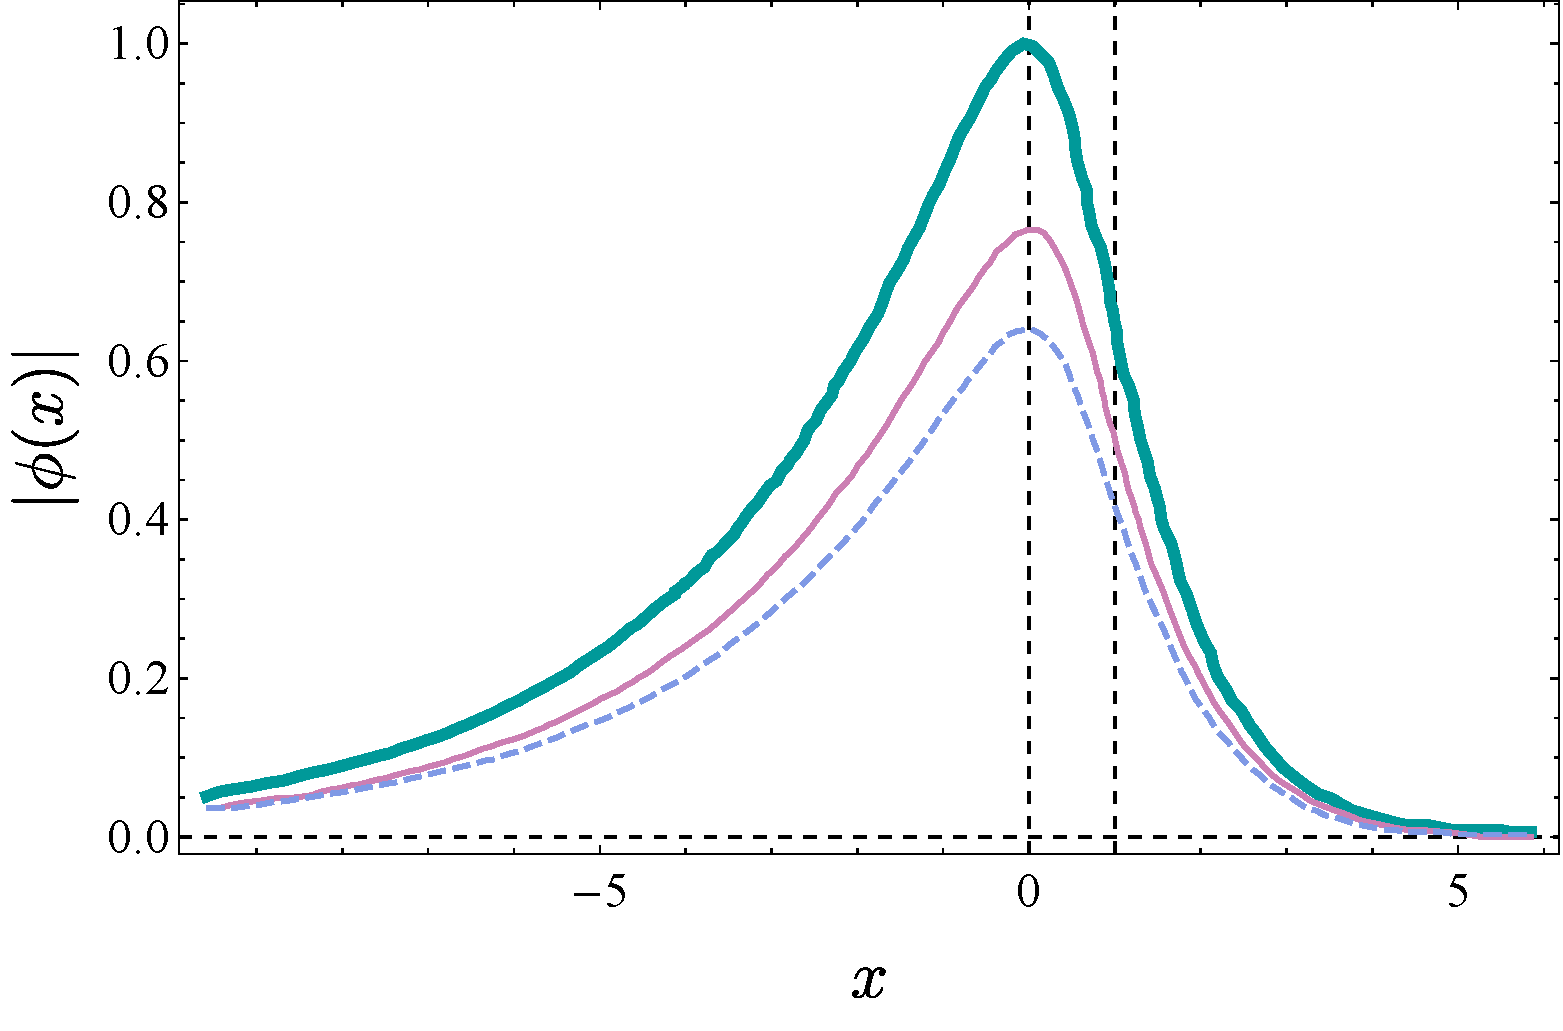
\includegraphics[width=7cm]{f36b}
\end{minipage}\\[20pt]                 
\caption{Campo cuántico $\phi(x)$ para una cavidad formada entre $x=0$ y $x=L=1$. La gr\'{a}fica $|\phi(x)|$ (l\'{i}nea gruesa verde), $\text{Re}(\phi)$ ( l\'{i}nea delgada rosa), $\text{Im}(\phi)$ ( l\'{i}nea discontinua azul) para $v_2=-2$ (izquierda) y $v_2 = -3$ (derecha) \citep{2018Bermudez}.}\label{fig:3.7}   
\end{figure}
\end{center}

Ahora, se necesita verificar que el comportamiento cualitativo de esta nueva solución compleja es soluci\'{o}n del problema planteado. En particular, se necesita verificar que los modos decaen de forma correcta en ambos lados de la cavidad. De los ocho valores de $\textbf{k}_1$ y $\textbf{k}_2$ mostrados en la figura \ref{fig:3.8}, donde  $\text{Re}(\omega_l)$ se deja fija y se cambia suavemente la parte imaginaria de la frecuencia de $0$ a $\text{Im}(\omega_l)$, nos interesan para ver el comportamiento asint\'{o}tico de la soluci\'{o}n aquellos modos que se encuentran en la regi\'{o}n subs\'{o}nica. De la ec. (\ref{prueba1}) la parte imaginaria del n\'{u}mero de onda domina el comportamiento asint\'{o}tico de la soluci\'{o}n, por tanto, los modos $k_{\text{1u}}$ y $k_{\text{1ul}}$ con parte imaginaria del n\'{u}mero de onda mayor que cero deben existir en la regi\'{o}n III, mientras que para los modos $k_{\text{1ul}}$ y $k_{\text{1v}}$ con parte  imaginaria en el n\'{u}mero de onda menor que cero deben existir solo en la regi\'{o}n I. Esta informaci\'{o}n es congruente con las condiciones impuestas a los coeficientes \textbf{A} y \textbf{C} en la figura \ref{fig:3.6}.\\

La forma en que decae el campo $\phi(x)$ mostrado en la figura \ref{fig:3.7} indica que la radiaci\'{o}n se est\'a propagando fuera de la cavidad.  Adem\'{a}s, dicho campo muestra una asim\'{e}tria  en la parte espacial: la mayor parte de la radiaci\'{o}n se propaga en la misma direcci\'{o}n en la que se propaga el flujo de fondo. Por ejemplo, para $v_1=-1/2$ y $v_2=-3$, los coeficientes fuera de la cavidad para un modo del l\'{a}ser son $\textbf{A}=(0,0,-1.2149+i0.3174,5.1095+i3.9008)$ en la regi\'{o}n I, y $\textbf{C}=(1,1.1497+i0.3824,0,0)$ en la regi\'{o}n III. Esto muestra que la radiación transplanckiana en el modo $k_{\text{1v}}$, con amplitud $A_4$, logra escapar del BHL, producto del tunelamiento del campo que se encuentra dentro de la cavidad. Este \'{u}ltimo comportamiento es t\'ipico de la RH, que es  radiaci\'{o}n que logra escapar de los horizontes.\\
 
Num\'{e}ricamente, se puede encontrar 
una \'{u}nica soluci\'{o}n (una sola frecuencia $\omega_l$) para las velocidades supersónicas cercanas a la velocidad trans\'{o}nica $v_t$, por ejemplo para $v_2=-3$. 
Sin embargo, podemos encontrar m\'{a}s soluciones si se eligen valores m\'{a}s negativos, por ejemplo para $v_2=-5$ hay dos soluciones. Esto genera de forma inmediata una pregunta: ¿es posible saber cu\'{a}ntas soluciones se pueden encontrar para un valor arbitrario de $v_2$? En la siguiente sección compararemos las soluciones encontradas a través de la teoría de
inestabilidades con un modelo simple, respondiendo con esto la pregunta antes mencionada.

\begin{figure}\centering
	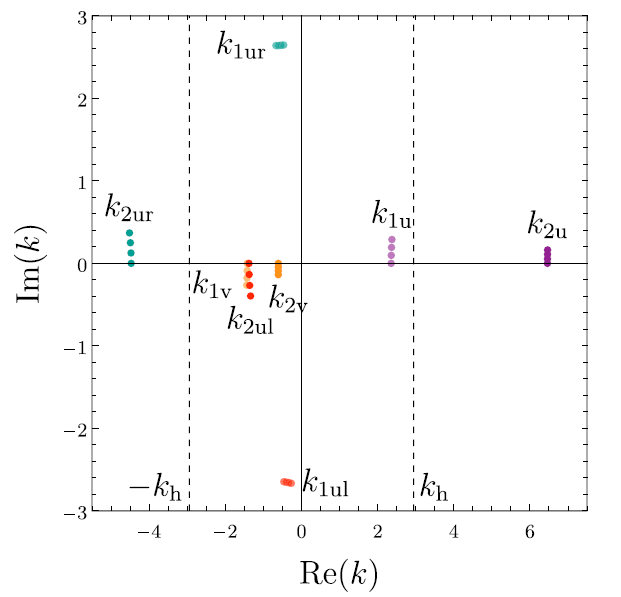
\includegraphics[scale=0.7]{F37}
	\caption{Cambio de $\textbf{k}_1$ y $\textbf{k}_2$ para $\text{Re}(\omega_l)$ fijo, e incrementando el valor de $\text{Im}(\omega)$ de $0$ a $\text{Im}(\omega_l)$ en peque\~{n}os pasos para $v_1=-1/2$ y $v_2=-3$ \citep{2018Bermudez}.}\label{fig:3.8}
\end{figure}

\section{Comparaci\'{o}n del modelo de inestabilidades con el m\'{e}todo simple}
En la secci\'{o}n anterior se mostr\'{o} que por teor\'{i}a de inestabilidades se pueden encontrar los modos del BHL. Variando $v_1$ y $v_2$ para un $L$ fijo se encuentra num\'{e}ricamente las soluciones para uno o m\'{a}s modos. Ahora se usar\'{a} un modelo simple para obtener una mejor imagen de la dinámica de los modos láser $k(\omega_l)$ con frecuencia compleja $\omega_l=\omega_R+i\omega_I$, pero considerando que $\omega_I\rightarrow 0$, que es la versi\'{o}n de una inestabilidad neutra o un modelo de onda plana con números de onda reales $k(\omega_R)$.\\

Recordando que en la evoluci\'{o}n usual de los modos del BHL (ver las secciones \ref{BHL} y  \ref{sec:real}), dos de los modos atrapados en la cavidad son $k_{\text{2ul}}$ que se mueve hacia la izquierda y $k_{\text{2ur}}$ que se mueve hacia la derecha en el marco com\'{o}vil los cuales permiten la creaci\'{o}n en cada ciclo de un modo $k_{\text{1u}}$ que logra salir de la cavidad, adem\'{a}s en cada \textit{rebote} con los horizontes se logra amplificar la radiaci\'{o}n que se encuentra en la configuraci\'{o}n del BHL. Con el modelo de ondas planas se puede demostrar que las soluciones de número de onda $k_{\text{2ul}}$ y  $k_{\text{2ur}}$ siguen una condición de resonancia en cada ciclo \citep{Leonhardt2007}.

\begin{figure}\centering
	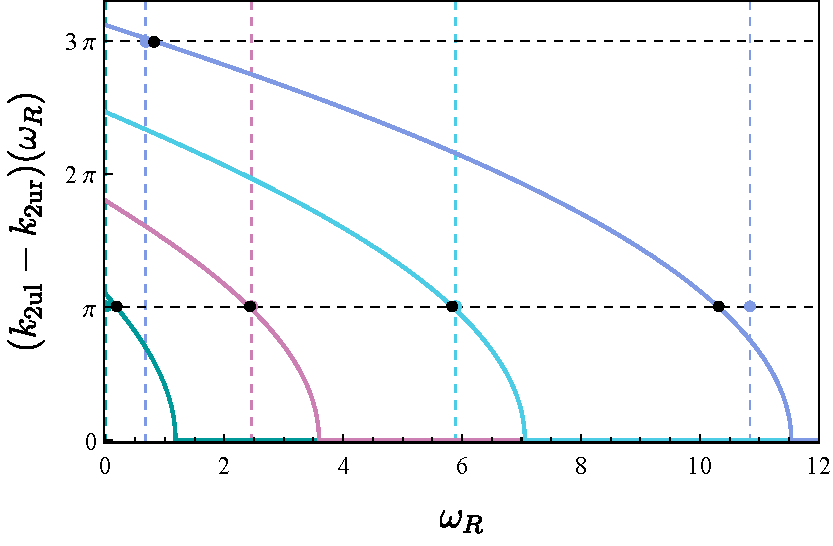
\includegraphics[scale=0.7]{F39}
	\caption{Diferencia de fase $(k_{\text{2ul}}-k_{\text{2ur}})(\omega_R)$ considerando el modelo de onda plana para $v_2=\{-2(\text{verde}), -3(\text{rosa}), -4 (\text{azul}),-5(\text{morado})\}$. Las diferencias de fase de $\pi$ y $3\pi$ predichas por el modelo están marcados por puntos negros. Las líneas discontinuas verticales marcan el valor de $\omega_R$ encontrado por la teoría de inestabilidades y su intersección con la fase son los puntos de color.}\label{fig:3.9}
\end{figure}

\subsection{Condici\'{o}n de resonancia}
Se produce una resonancia cuando la diferencia de fase de la radiación atrapada después de un ciclo ida y vuelta es un múltiplo entero de $2\pi$. Además, se producen dos reflexiones en los horizontes durante cada ciclo con un cambio de fase de $\pi/2$ cada uno. Entonces, la diferencia de fase entre los modos atrapados $ k_{\text{2ul}}$ y $k_{\text{2ur}}$ debería ser
$\Delta k L=(2n+1)\pi$, (con $L=1$). En la figura \ref{fig:3.9} se muestra la diferencia de fase $(\Delta k =k_{\text{2ul}} - k_{\text{2ur}})$ con el modelo de ondas neutras ($\omega_I=0$) para diferentes valores de $v_2$. Los puntos negros en la figura \ref{fig:3.9} indican las prediciones para $\omega_R$ del modelo simple, mientras los puntos de color que son las intersecciones entre las lineas verticales y discontinuas horizontales son las predicciones del modelo de inestabilidades.\\
Todas las predicciones del modelo simple son cercanas a los resutados encontrados con el modelo de frecuencias complejas, los valores difieren por un error menor a $10\%$. Esto significa que el modelo de onda plana para frecuencias reales es lo suficientemente bueno como para darnos una aproximación a la parte real de $\omega_l$. Además, refuerza la interpretación dada de la solución  con frecuencias complejas para el campo $\phi(x)$ obtenido en la secci\'{o}n \ref{sec:compleja}. De hecho, se puede concluir que el continuo rebote de los modos $k_{\text{2ul}}$ y $k_{\text{2ur}}$ con los horizontes son los responsables de la amplificaci\'{o}n del campo confinado y a su vez esto es producto de una inestabilidad, i.e., de que el campo $\phi$ posea una frecuencia compleja donde su parte real es mayor que cero.\\

Los resultados obtenidos por teor\'{i}a de inestabilidades no solo logran obtener la condici\'{o}n de resonancia en una buena aproximaci\'{o}n con los resultados que se obtienen con el modelo simple, sino que adem\'{a}s predicen que hay modos que logran propagarse fuera de los horizontes de manera similar a la radiaci\'{o}n de Hawking expuesta en el cap\'{i}tulo \ref{cap1}. Para frecuencias reales estas ondas no podr\'{i}an escapar de la cavidad, pero cuando se generaliza el problema a poseer una inestabilidad espacio-temporal de forma natural aparece que los modos de la cavidad se amplifican en el tiempo y pueden \textit{tunelar} y alejarse de ella, un comportamiento t\'{i}pico de la RH, que es  radiaci\'{o}n que logra escapar de los horizontes.\\
